\section{Liquid Cooling}

\begin{itemize}
\item[\textbf{(info)}]
For systems designed to be liquid-cooled, there is an opportunity for large energy 
savings compared to air-cooled designs.  Since liquids have more heat capacity than 
air, smaller volumes can achieve the same level of cooling and can be transported 
with minimal energy use.  In addition, if heat can be removed through a fluid phase 
change, heat removal capacity is further increased.  By bringing the liquid closer 
to the heat source, effective cooling can be provided with higher temperature fluids.  
The higher temperature liquid cooling can be produced without the need for 
compressor-based cooling.

\item[\textbf{(info)}]
[Customer] will specify the type of liquid cooling systems contained within the datacenter.  
The range of liquid supply temperatures available in the center corresponding to 
ASHRAE-recommended classes (W1-W4) will be provided to the vendor.  

\item[\textbf{(info)}]
A traditional datacenter is cooled using compressor-based cooling (i.e., chillers or 
CRAC units) and additional heat rejection equipment such as cooling towers or dry coolers.  
These liquid-cooled systems operate within ASHRAE-recommended ranges W1 and W2.  Systems 
designed to operate in these ranges will have limited energy efficiency capability.

\item[\textbf{(important)}]
For improved energy efficiency and reduced capital expense, many datacenters can be 
operated without compressor-based cooling, by using cooling towers or dry coolers 
combined with water-side economizers. These datacenters can operate within the ASHRAE 
W3 range and accordingly, systems should be requested to operate in this range.

\item[\textbf{(enhancing)}]
In most locations, liquid cooling of up to 45\celsius~can be provided using dry coolers.  
The ASHRAE W4 classification was defined to accommodate this low energy form of cooling.  
For this type of infrastructure, ASHRAE W4 class should be requested.  

\item[\textbf{(info)}]
Parameters like pressure, flow rate, and water quality may also be specified by each site 
in its procurement documents.  ASHRAE provides guidance on these parameters, although 
they are not defined in this guideline. 
\end{itemize}
 
\section{Air Cooling}
\begin{itemize}
\item[\textbf{(info)}]
ASHRAE Thermal Guidelines (2011) define environmental classes that allow temperatures 
up to 40\celsius~and 45\celsius.  

Figure~\ref{fig:ITenviron} is a pschometric chart illustratiing these new environmental 
temperature and humidity limits along with the recommended limits.

\item[\textbf{(mandatory)}]
The system must be able to operate in a Class A1 environment.  

\item[\textbf{(important)}]
It is better to operate in a Class A2 environment (important) 

\item[\textbf{(enhancing)}]
All other things equal, it is best to operate in a Class A3 environment.
\end{itemize}

%INCLUDE FIG 5-1
\begin{figure}[htbp]
\centering
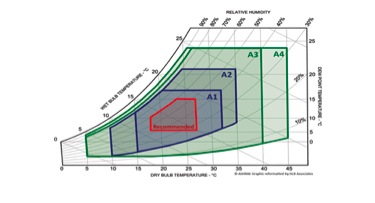
\includegraphics[width=5in]{fig2}
\caption{IT equipment environmental classes}
\label{fig:ITenviron}
\end{figure}

